\chapter{Propositional Logic: Reasoning with True and False}

\section{From Intuition to Formalism}

\begin{intuition}
In Chapter 1, we talked about mathematics as a game with symbols. Now we're going to play our first formal game: \textbf{propositional logic}.

This is logic at its simplest. We deal with statements that are either \textbf{true} or \textbf{false}, and we combine them using words like ``and,'' ``or,'' and ``not.''

Think of this as the foundation of all reasoning. Every time you say ``If it rains, then I'll bring an umbrella,'' you're using propositional logic.
\end{intuition}

\subsection{What Is a Proposition?}

Let's start with examples before we formalize.

\begin{example}[Propositions in Everyday Life]
These are propositions (statements with a definite true/false value):
\begin{itemize}
    \item ``The sky is blue'' (True)
    \item ``2 + 2 = 5'' (False)
    \item ``Paris is the capital of France'' (True)
    \item ``All cats are orange'' (False)
\end{itemize}

These are NOT propositions:
\begin{itemize}
    \item ``What time is it?'' (Question, not a statement)
    \item ``Close the door!'' (Command, not a statement)
    \item ``This sentence is false'' (Paradox---can't be consistently true or false)
    \item ``$x > 5$'' (Depends on $x$---not yet a proposition)
\end{itemize}
\end{example}

\begin{keyidea}
A proposition is a declarative statement that is either true or false (but not both, and not neither).

For now, think of propositions as sentences that make claims about the world. Later, we'll make this completely formal.
\end{keyidea}

\subsection{Building Complex Statements}

We can build complex propositions from simple ones using \textbf{logical connectives}:

\vspace{0.5cm}
\begin{center}
\begin{tikzpicture}[node distance=2.5cm]
    % Simple propositions
    \node[rectangle, draw, fill=blue!20, text width=4cm, align=center] (P) {$P$: ``It is raining''};
    \node[rectangle, draw, fill=blue!20, text width=4.5cm, align=center, right=of P] (Q) {$Q$: ``I have an umbrella''};
    
    % Complex propositions
    \node[rectangle, draw, fill=green!20, text width=5cm, align=center, below=2.5cm of P] (and) {
        $P \land Q$\\
        ``It is raining AND I have an umbrella''
    };
    
    \node[rectangle, draw, fill=green!20, text width=5.5cm, align=center, below=2.5cm of Q] (impl) {
        $P \implies Q$\\
        ``IF it is raining THEN I have an umbrella''
    };
    
    % Arrows
    \draw[->, thick] (P.south) -- (and.north) node[midway, left=0.2cm] {\small combine with};
    \draw[->, thick] (Q.south) -- (impl.north) node[midway, right=0.2cm] {\small connectives};
\end{tikzpicture}
\end{center}
\vspace{0.5cm}

Let's understand each connective intuitively before formalizing.

\subsection{The Five Connectives (Informally)}

\textbf{1. Negation ($\neg$): NOT}

$\neg P$ means ``not $P$'' or ``$P$ is false.''

\begin{example}
If $P$ = ``It is raining,'' then $\neg P$ = ``It is NOT raining.''

\vspace{0.5cm}
\begin{center}
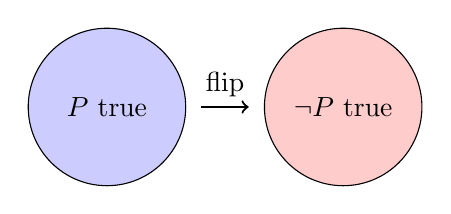
\begin{tikzpicture}
    \draw[fill=blue!20] (0,0) circle (1cm);
    \node at (0,0) {$P$ true};
    \draw[fill=red!20] (3,0) circle (1cm);
    \node at (3,0) {$\neg P$ true};
    \draw[->, thick] (1.2,0) -- (1.8,0) node[midway, above] {flip};
\end{tikzpicture}
\end{center}
\vspace{0.5cm}
\end{example}

\textbf{2. Conjunction ($\land$): AND}

$P \land Q$ means ``both $P$ and $Q$ are true.''

\begin{example}
$P$ = ``It is raining,'' $Q$ = ``It is cold''

$P \land Q$ = ``It is raining AND it is cold''

This is true only if BOTH conditions hold.

\vspace{0.5cm}
\begin{center}
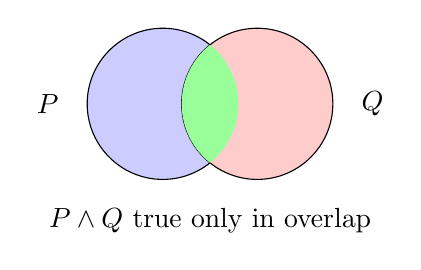
\begin{tikzpicture}[scale=0.8]
    % Venn diagram style
    \draw[fill=blue!20] (0,0) circle (1.2cm);
    \draw[fill=red!20] (1.5,0) circle (1.2cm);
    \node[left] at (-1.5,0) {$P$};
    \node[right] at (3,0) {$Q$};
    \node[below] at (0.75,-1.5) {$P \land Q$ true only in overlap};
    
    % Highlight intersection
    \begin{scope}
        \clip (0,0) circle (1.2cm);
        \fill[green!40] (1.5,0) circle (1.2cm);
    \end{scope}
\end{tikzpicture}
\end{center}
\vspace{0.5cm}
\end{example}

\textbf{3. Disjunction ($\lor$): OR}

$P \lor Q$ means ``at least one of $P$ or $Q$ is true'' (possibly both).

\begin{example}
$P$ = ``I will take the bus,'' $Q$ = ``I will take the train''

$P \lor Q$ = ``I will take the bus OR the train (or both if they go to the same place)''

This is true if either (or both) hold.
\end{example}

\begin{warning}
In everyday English, ``or'' sometimes means ``one but not both'' (exclusive or). In logic, $\lor$ means ``at least one'' (inclusive or). 

``Would you like coffee or tea?'' (English: exclusive)

``$x > 5$ or $x < 10$'' (Logic: inclusive---both could be true)
\end{warning}

\textbf{4. Implication ($\implies$): IF...THEN}

$P \implies Q$ means ``if $P$ is true, then $Q$ must be true.''

\begin{example}
$P$ = ``It is raining,'' $Q$ = ``The ground is wet''

$P \implies Q$ = ``If it is raining, then the ground is wet''
\end{example}

This is the trickiest connective! Let's understand it deeply:

\vspace{0.5cm}
\begin{center}
\begin{tikzpicture}[node distance=1.5cm]
    \node[rectangle, draw, fill=yellow!20, text width=3cm, align=center] (hyp) {$P$\\(hypothesis)};
    \node[rectangle, draw, fill=green!20, text width=3cm, align=center, right=3cm of hyp] (conc) {$Q$\\(conclusion)};
    \draw[->, ultra thick] (hyp) -- (conc) node[midway, above] {$\implies$};
    \node[below=0.4cm of hyp] {\small ``If this...''};
    \node[below=0.4cm of conc] {\small ``...then that''};
\end{tikzpicture}
\end{center}
\vspace{0.5cm}

\begin{keyidea}
The implication $P \implies Q$ is a \textbf{promise}: ``Whenever $P$ is true, $Q$ will also be true.''

The promise is \textbf{broken} only when $P$ is true but $Q$ is false. In all other cases, the promise holds.
\end{keyidea}

\textbf{5. Biconditional ($\iff$): IF AND ONLY IF}

$P \iff Q$ means ``$P$ and $Q$ always have the same truth value.''

\begin{example}
$P$ = ``$x = 2$,'' $Q$ = ``$x^2 = 4$''

$P \iff Q$ would mean these always happen together (which isn't quite true because $x = -2$ also makes $x^2 = 4$).

Better example:
$P$ = ``A triangle is equilateral,'' $Q$ = ``All three sides are equal''

$P \iff Q$ = true (these mean exactly the same thing)
\end{example}

\section{Making It Formal: Syntax}

Now that we have intuition, let's build the formal system.

\begin{keyidea}
Remember the pattern from Chapter 1:
\begin{enumerate}
    \item Define the \textbf{alphabet} (symbols we can use)
    \item Define which strings are \textbf{well-formed formulas} (grammatically correct)
    \item Define what formulas \textbf{mean} (semantics)
    \item Prove theorems about the system
\end{enumerate}

We're doing step 1 and 2 now: pure syntax.
\end{keyidea}

\subsection{The Alphabet of Propositional Logic}

\begin{definition}[Alphabet]
Our alphabet $\mathcal{L}_0$ consists of:
\begin{enumerate}
    \item \textbf{Propositional variables}: $P, Q, R, S, P_1, P_2, \ldots$ (infinitely many)
    \item \textbf{Logical connectives}: $\neg, \land, \lor, \implies, \iff$
    \item \textbf{Parentheses}: $($ and $)$
\end{enumerate}
\end{definition}

\begin{remark}
Propositional variables are placeholders for actual propositions. $P$ might stand for ``it is raining'' or ``$2 + 2 = 4$'' or anything with a truth value.
\end{remark}

\subsection{Well-Formed Formulas: What's Legal?}

Not every string of symbols makes sense. ``$\land \land P Q )$'' uses our symbols, but it's nonsense. We need rules for what's grammatically correct.

\begin{definition}[Well-Formed Formula]
The set of \textbf{well-formed formulas} (WFFs) is defined recursively:

\textbf{Base case:}
\begin{itemize}
    \item Every propositional variable ($P, Q, R, \ldots$) is a WFF
\end{itemize}

\textbf{Recursive rules:} If $\phi$ and $\psi$ are WFFs, then so are:
\begin{itemize}
    \item $(\neg \phi)$
    \item $(\phi \land \psi)$
    \item $(\phi \lor \psi)$
    \item $(\phi \implies \psi)$
    \item $(\phi \iff \psi)$
\end{itemize}

\textbf{Nothing else is a WFF.}
\end{definition}

\begin{intuition}
Think of this as a recipe:
\begin{enumerate}
    \item Start with simple ingredients (variables)
    \item Combine them using approved methods (connectives)
    \item Keep combining what you've built
    \item You can only use what the rules allow
\end{enumerate}
\end{intuition}

\begin{example}[Building Formulas]
\textbf{Step-by-step construction:}

\textbf{Level 1:} $P, Q, R$ are WFFs (base case)

\textbf{Level 2:} Since $P$ and $Q$ are WFFs:
\begin{itemize}
    \item $(\neg P)$ is a WFF
    \item $(P \land Q)$ is a WFF
    \item $(P \lor Q)$ is a WFF
\end{itemize}

\textbf{Level 3:} Since $(P \land Q)$ and $R$ are WFFs:
\begin{itemize}
    \item $((P \land Q) \implies R)$ is a WFF
\end{itemize}
\end{example}

\vspace{0.5cm}
\begin{center}
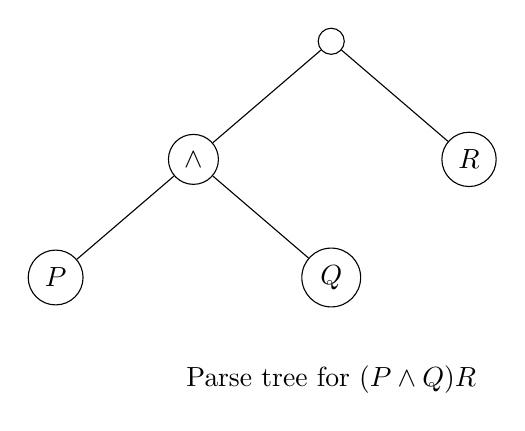
\begin{tikzpicture}[level distance=1.5cm, sibling distance=3.5cm]
    \node[circle, draw] {$\implies$}
        child {node[circle, draw] {$\land$}
            child {node[circle, draw] {$P$}}
            child {node[circle, draw] {$Q$}}
        }
        child {node[circle, draw] {$R$}};
    \node[below=1.5cm] at (0,-2.5) {Parse tree for $(P \land Q) \implies R$};
\end{tikzpicture}
\end{center}
\vspace{0.5cm}

\begin{example}[What's NOT a WFF]
\begin{itemize}
    \item $P \land$ --- incomplete
    \item $\land P Q$ --- wrong structure (prefix notation not allowed)
    \item $P Q$ --- missing connective
    \item $(P \land)$ --- incomplete
\end{itemize}
\end{example}

\subsection{Precedence Rules (Practical Notation)}

Writing all those parentheses gets tedious. We adopt conventions:

\begin{notation}[Precedence]
\begin{enumerate}
    \item $\neg$ binds tightest (apply first)
    \item $\land$ and $\lor$ bind next
    \item $\implies$ and $\iff$ bind weakest (apply last)
\end{enumerate}

So $\neg P \land Q \implies R$ means $((\neg P) \land Q) \implies R$.
\end{notation}

\vspace{0.5cm}
\begin{center}
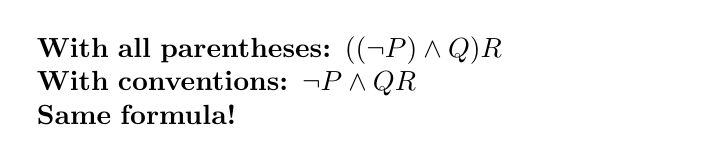
\begin{tikzpicture}
    \node[text width=8cm] {
        \textbf{With all parentheses:} $((\neg P) \land Q) \implies R$\\
        \textbf{With conventions:} $\neg P \land Q \implies R$\\
        \textbf{Same formula!}
    };
\end{tikzpicture}
\end{center}
\vspace{0.5cm}

\section{Giving Meaning: Semantics}

We've defined which strings are grammatically correct. Now: \textit{what do they mean?}

\subsection{Truth Values}

\begin{definition}[Truth Values]
We work with two truth values: $\mathbb{B} = \{0, 1\}$ where:
\begin{itemize}
    \item $0$ represents ``false''
    \item $1$ represents ``true''
\end{itemize}
\end{definition}

\begin{remark}
We use $0$ and $1$ (instead of $F$ and $T$) to emphasize these are just formal objects. We could use any two distinct symbols. The labels ``false'' and ``true'' are just convenient names.
\end{remark}

\subsection{Truth Assignments}

\begin{definition}[Truth Assignment]
A \textbf{truth assignment} (or \textbf{valuation}) is a function:
\[v: \{\text{propositional variables}\} \to \{0, 1\}\]
that assigns a truth value to each propositional variable.
\end{definition}

\begin{intuition}
A truth assignment is a ``possible world.'' It says: in this scenario, $P$ is true, $Q$ is false, $R$ is true, etc.

Example scenarios:
\begin{itemize}
    \item $v_1$: $P \mapsto 1, Q \mapsto 0, R \mapsto 1$ (``$P$ and $R$ are true, $Q$ is false'')
    \item $v_2$: $P \mapsto 0, Q \mapsto 0, R \mapsto 0$ (``everything is false'')
    \item $v_3$: $P \mapsto 1, Q \mapsto 1, R \mapsto 1$ (``everything is true'')
\end{itemize}
\end{intuition}

\vspace{0.5cm}
\begin{center}
\begin{tikzpicture}
    \node[rectangle, draw, fill=yellow!20, text width=3cm, align=center] (vars) {Variables\\$P, Q, R, \ldots$};
    \node[rectangle, draw, fill=blue!20, text width=3cm, align=center, right=3cm of vars] (vals) {Truth Values\\$\{0, 1\}$};
    \draw[->, thick] (vars) -- (vals) node[midway, above] {$v$} node[midway, below] {\small (valuation)};
\end{tikzpicture}
\end{center}
\vspace{0.5cm}

\subsection{Truth Functions: How Connectives Work}

Now we extend the valuation to \textit{all} formulas by defining how connectives combine truth values.

\begin{definition}[Truth Functions]
For any valuation $v$ and formulas $\phi, \psi$:

\textbf{Negation:}
\[v(\neg \phi) = \begin{cases} 1 & \text{if } v(\phi) = 0 \\ 0 & \text{if } v(\phi) = 1 \end{cases}\]

\textbf{Conjunction:}
\[v(\phi \land \psi) = \begin{cases} 1 & \text{if } v(\phi) = 1 \text{ and } v(\psi) = 1 \\ 0 & \text{otherwise} \end{cases}\]

\textbf{Disjunction:}
\[v(\phi \lor \psi) = \begin{cases} 1 & \text{if } v(\phi) = 1 \text{ or } v(\psi) = 1 \text{ (or both)} \\ 0 & \text{otherwise} \end{cases}\]

\textbf{Implication:}
\[v(\phi \implies \psi) = \begin{cases} 0 & \text{if } v(\phi) = 1 \text{ and } v(\psi) = 0 \\ 1 & \text{otherwise} \end{cases}\]

\textbf{Biconditional:}
\[v(\phi \iff \psi) = \begin{cases} 1 & \text{if } v(\phi) = v(\psi) \\ 0 & \text{otherwise} \end{cases}\]
\end{definition}

Let's visualize these with truth tables.

\subsection{Truth Tables}

A \textbf{truth table} shows the output for all possible inputs.

\textbf{Negation:}
\begin{center}
{\renewcommand{\arraystretch}{1.3}
\begin{tabular}{c|c}
\hline
$P$ & $\neg P$ \\ \hline
0 & 1 \\
1 & 0 \\
\end{tabular}}
\end{center}

\begin{intuition}
Negation flips the truth value. Simple!
\end{intuition}

\textbf{Conjunction (AND):}
\begin{center}
{\renewcommand{\arraystretch}{1.3}
\begin{tabular}{cc|c}
\hline
$P$ & $Q$ & $P \land Q$ \\ \hline
0 & 0 & 0 \\
0 & 1 & 0 \\
1 & 0 & 0 \\
1 & 1 & 1 \\
\end{tabular}}
\end{center}

\begin{intuition}
``AND'' is strict: true only when BOTH are true.
\end{intuition}

\textbf{Disjunction (OR):}
\begin{center}
{\renewcommand{\arraystretch}{1.3}
\begin{tabular}{cc|c}
\hline
$P$ & $Q$ & $P \lor Q$ \\ \hline
0 & 0 & 0 \\
0 & 1 & 1 \\
1 & 0 & 1 \\
1 & 1 & 1 \\
\end{tabular}}
\end{center}

\begin{intuition}
``OR'' is generous: true when AT LEAST ONE is true.
\end{intuition}

\textbf{Implication (IF...THEN):}
\begin{center}
{\renewcommand{\arraystretch}{1.3}
\begin{tabular}{cc|c}
\hline
$P$ & $Q$ & $P \implies Q$ \\ \hline
0 & 0 & 1 \\
0 & 1 & 1 \\
1 & 0 & 0 \\
1 & 1 & 1 \\
\end{tabular}}
\end{center}

This deserves special attention!

\begin{keyidea}
The implication $P \implies Q$ is false ONLY when the hypothesis ($P$) is true but the conclusion ($Q$) is false.

Why are rows 1 and 2 true (when $P$ is false)?

Think of it as a promise: ``If $P$ happens, then $Q$ will happen.''
\begin{itemize}
    \item If $P$ doesn't happen, the promise isn't tested---we consider it kept.
    \item This is called \textbf{vacuous truth}: an implication with false hypothesis is vacuously true.
\end{itemize}
\end{keyidea}

\begin{example}[Vacuous Truth]
``If $1 = 0$, then pigs can fly.''

The hypothesis ($1 = 0$) is false. So this entire statement is \textit{vacuously true}!

Weird? Yes. But consistent? Absolutely. This definition makes mathematical theorems work correctly.
\end{example}

\vspace{0.5cm}
\begin{center}
\begin{tikzpicture}[scale=0.9]
    \node[text width=10cm] {
        \textbf{Why this definition?}\\[0.3cm]
        Consider: ``If it rains, the ground is wet.''\\[0.2cm]
        Four scenarios:\\[0.2cm]
        \textbf{1.} Rain + wet ground: Promise kept ✓ (true)\\
        \textbf{2.} Rain + dry ground: Promise broken ✗ (false)\\
        \textbf{3.} No rain + wet ground: Promise not tested ✓ (true)\\
        \textbf{4.} No rain + dry ground: Promise not tested ✓ (true)
    };
\end{tikzpicture}
\end{center}
\vspace{0.5cm}

\textbf{Biconditional (IF AND ONLY IF):}
\begin{center}
{\renewcommand{\arraystretch}{1.3}
\begin{tabular}{cc|c}
\hline
$P$ & $Q$ & $P \iff Q$ \\ \hline
0 & 0 & 1 \\
0 & 1 & 0 \\
1 & 0 & 0 \\
1 & 1 & 1 \\
\end{tabular}}
\end{center}

\begin{intuition}
$P \iff Q$ means ``$P$ and $Q$ always go together.'' True when both have the same value.
\end{intuition}

\section{Important Formulas and Equivalences}

Now we can state and prove general laws.

\subsection{Tautologies: Always True}

\begin{definition}[Tautology]
A formula $\phi$ is a \textbf{tautology} if $v(\phi) = 1$ for \textit{every} valuation $v$.

We write $\models \phi$ to mean ``$\phi$ is a tautology.''
\end{definition}

\begin{intuition}
A tautology is \textit{logically true}---true regardless of what propositions mean. It's true purely because of its logical structure.
\end{intuition}

\begin{example}[Famous Tautologies]
\begin{enumerate}
    \item \textbf{Law of Excluded Middle}: $P \lor \neg P$
    
    ``Either $P$ is true or $P$ is false.'' (No middle option!)
    
    \begin{center}
    {\renewcommand{\arraystretch}{1.3}
    \begin{tabular}{c|c|c}
    \hline
    $P$ & $\neg P$ & $P \lor \neg P$ \\ \hline
    0 & 1 & 1 \\
    1 & 0 & 1 \\
    \end{tabular}}
    \end{center}
    
    Always true! ✓
    
    \item \textbf{Law of Non-Contradiction}: $\neg(P \land \neg P)$
    
    ``$P$ can't be both true and false.''
    
    \item \textbf{Identity}: $P \implies P$
    
    ``If $P$ is true, then $P$ is true.'' (Trivial but fundamental!)
\end{enumerate}
\end{example}

\subsection{Key Logical Equivalences}

\begin{definition}[Logical Equivalence]
Formulas $\phi$ and $\psi$ are \textbf{logically equivalent} (written $\phi \equiv \psi$) if they have identical truth tables---that is, $v(\phi) = v(\psi)$ for all valuations $v$.
\end{definition}

\begin{theorem}[Fundamental Equivalences]
The following equivalences hold:

\textbf{1. Double Negation:}
\[\neg \neg P \equiv P\]

\textbf{2. Commutativity:}
\begin{align*}
P \land Q &\equiv Q \land P \\
P \lor Q &\equiv Q \lor P
\end{align*}

\textbf{3. Associativity:}
\begin{align*}
(P \land Q) \land R &\equiv P \land (Q \land R) \\
(P \lor Q) \lor R &\equiv P \lor (Q \lor R)
\end{align*}

\textbf{4. Distributivity:}
\begin{align*}
P \land (Q \lor R) &\equiv (P \land Q) \lor (P \land R) \\
P \lor (Q \land R) &\equiv (P \lor Q) \land (P \lor R)
\end{align*}

\textbf{5. De Morgan's Laws:}
\begin{align*}
\neg(P \land Q) &\equiv \neg P \lor \neg Q \\
\neg(P \lor Q) &\equiv \neg P \land \neg Q
\end{align*}

\textbf{6. Implication as Disjunction:}
\[P \implies Q \equiv \neg P \lor Q\]

\textbf{7. Contrapositive:}
\[P \implies Q \equiv \neg Q \implies \neg P\]
\end{theorem}

Let me prove a few to show the method:

\begin{proof}[Proof of De Morgan's Law: $\neg(P \land Q) \equiv \neg P \lor \neg Q$]

We show these have identical truth tables:

\begin{center}
{\renewcommand{\arraystretch}{1.3}
\begin{tabular}{cc|c|cc|c}
\hline
$P$ & $Q$ & $P \land Q$ & $\neg(P \land Q)$ & $\neg P \lor \neg Q$ & Match? \\ \hline
0 & 0 & 0 & 1 & 1 & ✓ \\
0 & 1 & 0 & 1 & 1 & ✓ \\
1 & 0 & 0 & 1 & 1 & ✓ \\
1 & 1 & 1 & 0 & 0 & ✓ \\
\end{tabular}}
\end{center}

Columns match exactly! Therefore $\neg(P \land Q) \equiv \neg P \lor \neg Q$.
\end{proof}

\begin{intuition}
De Morgan's Laws say: to negate an ``and,'' flip to ``or'' and negate each part. To negate an ``or,'' flip to ``and'' and negate each part.

\textbf{Example:} Negate ``It's raining AND cold''
\begin{itemize}
    \item Becomes: ``It's NOT raining OR it's NOT cold''
    \item Makes sense: the original is false if at least one condition fails
\end{itemize}
\end{intuition}

\begin{proof}[Proof of Contrapositive: $P \implies Q \equiv \neg Q \implies \neg P$]

\begin{center}
{\renewcommand{\arraystretch}{1.3}
\begin{tabular}{cc|c|cc|c}
\hline
$P$ & $Q$ & $P \implies Q$ & $\neg Q$ & $\neg P$ & $\neg Q \implies \neg P$ \\ \hline
0 & 0 & 1 & 1 & 1 & 1 \\
0 & 1 & 1 & 0 & 1 & 1 \\
1 & 0 & 0 & 1 & 0 & 0 \\
1 & 1 & 1 & 0 & 0 & 1 \\
\end{tabular}}
\end{center}

Columns 3 and 6 match! Therefore $P \implies Q \equiv \neg Q \implies \neg P$.
\end{proof}

\begin{keyidea}
The contrapositive is \textit{logically identical} to the original implication. This is why proof by contrapositive works:

To prove ``$P \implies Q$,'' we can instead prove ``$\neg Q \implies \neg P$.'' Same thing!

\textbf{Example:} 
\begin{itemize}
    \item Original: ``If $n^2$ is even, then $n$ is even''
    \item Contrapositive: ``If $n$ is odd, then $n^2$ is odd''
    \item (The contrapositive is often easier to prove!)
\end{itemize}
\end{keyidea}

\section{Inference Rules: How We Reason}

Now we can formalize common patterns of reasoning.

\subsection{Modus Ponens}

\begin{theorem}[Modus Ponens]
\[(P \land (P \implies Q)) \implies Q \text{ is a tautology}\]
\end{theorem}

\begin{intuition}
\textbf{In words:} ``If $P$ is true, and if '$P$ implies $Q$' is true, then $Q$ must be true.''

\textbf{Pattern of reasoning:}
\begin{enumerate}
    \item We know $P$ is true
    \item We know $P \implies Q$ is true
    \item Therefore, $Q$ must be true
\end{enumerate}

This is the most fundamental rule of inference!
\end{intuition}

\vspace{0.5cm}
\begin{center}
\begin{tikzpicture}[node distance=0.8cm]
    \node[rectangle, draw, fill=blue!20, minimum width=3cm] (p) {$P$};
    \node[rectangle, draw, fill=blue!20, minimum width=3cm, below=of p] (pq) {$P \implies Q$};
    \node[rectangle, draw, fill=green!20, minimum width=3cm, below=1.2cm of pq] (q) {$\therefore Q$};
    
    % Horizontal line separating premises from conclusion
    \draw[thick] ($(pq.south west) + (-0.8, -0.6)$) -- ($(pq.south east) + (0.8, -0.6)$);
    
    % Premises text aligned with top boxes
    \node[right=2.5cm of p, text width=4.5cm, align=left, anchor=north west] {
        \textbf{Premises:}\\
        We have $P$\\
        We have $P \implies Q$
    };
    
    % Conclusion text aligned with bottom box
    \node[right=2.5cm of q, text width=4.5cm, align=left] {
        \textbf{Conclusion:}\\
        Therefore we conclude $Q$
    };
\end{tikzpicture}
\end{center}
\vspace{0.5cm}

\subsection{Other Inference Rules}

\begin{theorem}[Modus Tollens]
\[((P \implies Q) \land \neg Q) \implies \neg P \text{ is a tautology}\]
\end{theorem}

\begin{intuition}
``If $P \implies Q$ is true, and $Q$ is false, then $P$ must be false.''

Why? If $P$ were true, then $Q$ would have to be true (by the implication). But $Q$ is false. Contradiction! So $P$ must be false.
\end{intuition}

\begin{theorem}[Hypothetical Syllogism]
\[((P \implies Q) \land (Q \implies R)) \implies (P \implies R) \text{ is a tautology}\]
\end{theorem}

\begin{intuition}
``Implications chain.'' If $P$ leads to $Q$, and $Q$ leads to $R$, then $P$ leads to $R$.

\vspace{0.5cm}
\begin{center}
\begin{tikzpicture}
    \node[circle, draw] (p) {$P$};
    \node[circle, draw, right=2cm of p] (q) {$Q$};
    \node[circle, draw, right=2cm of q] (r) {$R$};
    \draw[->, thick] (p) -- (q);
    \draw[->, thick] (q) -- (r);
    \draw[->, thick, red, bend right=40] (p) to node[below] {therefore} (r);
\end{tikzpicture}
\end{center}
\vspace{0.5cm}
\end{intuition}

\section{Predicate Logic: The Language of Quantifiers}

\begin{intuition}
Propositional logic is great, but it's not enough. Consider this classic argument:
\begin{enumerate}
    \item All men are mortal.
    \item Socrates is a man.
    \item Therefore, Socrates is mortal.
\end{enumerate}

In propositional logic, this looks like:
\begin{enumerate}
    \item $P$ (``All men are mortal'')
    \item $Q$ (``Socrates is a man'')
    \item Therefore $R$ (``Socrates is mortal'')
\end{enumerate}
There is no logical link between $P$, $Q$, and $R$! To see the connection, we need to look \textit{inside} the propositions. We need \textbf{Predicate Logic}.
\end{intuition}

\subsection{Predicates and Variables}

\begin{definition}[Predicate]
A \textbf{predicate} is a statement involving variables (like $x, y$) that becomes a proposition (true or false) when specific values are substituted for the variables.
\end{definition}

\begin{example}
Let $P(x)$ be the statement ``$x > 5$''.
\begin{itemize}
    \item $P(x)$ is not true or false (it depends on $x$).
    \item $P(2)$ is ``$2 > 5$'', which is \textbf{false}.
    \item $P(7)$ is ``$7 > 5$'', which is \textbf{true}.
\end{itemize}
\end{example}

\subsection{Quantifiers}

We can also make a predicate into a proposition by quantifying over a \textbf{domain of discourse} (the set of all objects we are talking about).

\begin{definition}[Universal Quantifier $\forall$]
The symbol $\forall$ means ``for all'' or ``for every''.
\[ \forall x P(x) \]
means ``for every $x$ in the domain, $P(x)$ is true.''
\end{definition}

\begin{definition}[Existential Quantifier $\exists$]
The symbol $\exists$ means ``there exists'' or ``for some''.
\[ \exists x P(x) \]
means ``there is at least one $x$ in the domain such that $P(x)$ is true.''
\end{definition}

\begin{example}
Domain: integers $\mathbb{Z}$. Let $P(x)$ be ``$x^2 \ge 0$''.
\begin{itemize}
    \item $\forall x P(x)$ is true (square of any integer is non-negative).
    \item $\exists x (x < 0)$ is true (e.g., $-1$).
    \item $\forall x (x > 0)$ is false (e.g., $-1$ is not $> 0$).
\end{itemize}
\end{example}

\subsection{Negating Quantifiers (De Morgan for Logic)}

How do we say ``Not everyone likes pizza''?
It means ``There exists someone who does \textbf{not} like pizza.''

\begin{theorem}[De Morgan's Laws for Quantifiers]
\begin{align*}
\neg (\forall x P(x)) &\equiv \exists x \neg P(x) \\
\neg (\exists x P(x)) &\equiv \forall x \neg P(x)
\end{align*}
\end{theorem}

\begin{intuition}
To show a universal statement (``All swans are white'') is false, you only need to find \textbf{one} counterexample (one black swan). You don't need to show \textit{all} swans are non-white.
\end{intuition}

\subsection{Bounded Quantifiers}\index{bounded quantifiers}\index{quantifiers!bounded}

\begin{keyidea}
In set theory and mathematics, we often quantify over elements of a specific set, not over all objects. This leads to \textbf{bounded quantifiers} (also called \textbf{restricted quantifiers}).
\end{keyidea}

\begin{definition}[Bounded Quantifier Notation]
The notation $\forall x \in A, P(x)$ and $\exists x \in A, P(x)$ are \textbf{abbreviations}:

\begin{align*}
\forall x \in A, P(x) &\equiv \forall x (x \in A \implies P(x)) \\
\exists x \in A, P(x) &\equiv \exists x (x \in A \land P(x))
\end{align*}

\textbf{In words:}
\begin{itemize}
    \item $\forall x \in A, P(x)$: ``For all $x$ in $A$, $P(x)$ holds'' means ``If $x$ is in $A$, then $P(x)$''
    \item $\exists x \in A, P(x)$: ``There exists $x$ in $A$ such that $P(x)$'' means ``There exists $x$ that is both in $A$ and satisfies $P(x)$''
\end{itemize}
\end{definition}

\begin{example}[Bounded vs. Unbounded Quantifiers]
\textbf{Unbounded}: $\forall x (x^2 \geq 0)$ --- quantifies over all objects

\textbf{Bounded}: $\forall x \in \mathbb{R}, x^2 \geq 0$ --- quantifies only over real numbers

Expanded form: $\forall x (x \in \mathbb{R} \implies x^2 \geq 0)$

\vspace{0.5cm}

\textbf{Unbounded}: $\exists x (x^2 = 2)$ --- might not have a solution depending on universe

\textbf{Bounded}: $\exists x \in \mathbb{R}, x^2 = 2$ --- solution exists in the reals

Expanded form: $\exists x (x \in \mathbb{R} \land x^2 = 2)$
\end{example}

\begin{warning}
Notice the asymmetry:
\begin{itemize}
    \item Universal bounded quantifiers use $\implies$ (implication)
    \item Existential bounded quantifiers use $\land$ (conjunction)
\end{itemize}

This is correct! Think about it: ``All reals are positive'' is false if even one real is non-positive (implication handles this). But ``There exists a positive real'' needs to find something that is \textit{both} real \textit{and} positive (conjunction).
\end{warning}

\begin{remark}
Throughout this text, when we move from logic to set theory and beyond, we will frequently use bounded quantifier notation. Remember that these are always translatable back to pure first-order logic using the definitions above.
\end{remark}

\section{First-Order Logic: Formal Syntax}\index{first-order logic}\index{predicate logic}

Now we make predicate logic completely formal, just as we did for propositional logic.

\subsection{The Language of First-Order Logic}\index{first-order logic!syntax}

\begin{definition}[Alphabet of First-Order Logic]
The alphabet consists of:
\begin{enumerate}
    \item \textbf{Variables}: $x, y, z, x_1, x_2, \ldots$ (infinitely many)
    \item \textbf{Logical connectives}: $\neg, \land, \lor, \implies, \iff$
    \item \textbf{Quantifiers}: $\forall$ (universal), $\exists$ (existential)
    \item \textbf{Equality}: $=$ (optional, depending on context)
    \item \textbf{Parentheses}: $(, )$
    \item \textbf{Non-logical symbols} (vary by application):
    \begin{itemize}
        \item \textbf{Constant symbols}: $c, d, 0, 1, \ldots$
        \item \textbf{Function symbols}: $f, g, +, \times, \ldots$ (each has arity)
        \item \textbf{Predicate symbols}: $P, Q, <, \in, \ldots$ (each has arity)
    \end{itemize}
\end{enumerate}
\end{definition}

\begin{example}[Language of Arithmetic]
For Peano arithmetic:
\begin{itemize}
    \item Constant: $0$
    \item Functions: $S$ (successor, arity 1), $+$ (addition, arity 2), $\times$ (multiplication, arity 2)
    \item Predicate: $=$ (equality, arity 2)
\end{itemize}

Example formula: $\forall x \exists y (x + S(0) = y)$ (``for every $x$, there exists $y$ such that $x + 1 = y$'')
\end{example}

\subsection{Terms and Formulas}\index{first-order logic!terms}\index{first-order logic!formulas}

\begin{definition}[Terms]
\textbf{Terms} are built recursively:
\begin{enumerate}
    \item Every variable is a term
    \item Every constant symbol is a term
    \item If $t_1, \ldots, t_n$ are terms and $f$ is a function symbol of arity $n$, then $f(t_1, \ldots, t_n)$ is a term
\end{enumerate}

Terms represent objects in the domain.
\end{definition}

\begin{definition}[Well-Formed Formulas (WFFs) of First-Order Logic]
The set of well-formed formulas is defined recursively:

\textbf{Base case (Atomic formulas):}
\begin{itemize}
    \item If $P$ is a predicate symbol of arity $n$ and $t_1, \ldots, t_n$ are terms, then $P(t_1, \ldots, t_n)$ is a WFF
    \item If $t_1$ and $t_2$ are terms, then $(t_1 = t_2)$ is a WFF
\end{itemize}

\textbf{Recursive rules:} If $\phi$ and $\psi$ are WFFs and $x$ is a variable:
\begin{itemize}
    \item $(\neg \phi)$ is a WFF
    \item $(\phi \land \psi)$, $(\phi \lor \psi)$, $(\phi \implies \psi)$, $(\phi \iff \psi)$ are WFFs
    \item $(\forall x \phi)$ is a WFF
    \item $(\exists x \phi)$ is a WFF
\end{itemize}
\end{definition}

\begin{example}[Building a Formula]
Domain: natural numbers. Build: ``Every number has a successor greater than itself''

\textbf{Step by step:}
\begin{enumerate}
    \item Atomic: $x < S(x)$ (``$x$ is less than the successor of $x$'')
    \item Quantify: $\forall x (x < S(x))$
\end{enumerate}

Full formula: $\forall x (x < S(x))$
\end{example}

\subsection{Free and Bound Variables}\index{free variable}\index{bound variable}

\begin{definition}[Free and Bound Variables]
In a formula $\phi$:
\begin{itemize}
    \item A variable $x$ is \textbf{bound} if it appears within the scope of a quantifier $\forall x$ or $\exists x$
    \item A variable $x$ is \textbf{free} if it is not bound
\end{itemize}

A formula with no free variables is called a \textbf{sentence}.
\end{definition}

\begin{example}
\begin{itemize}
    \item $\forall x P(x, y)$: $x$ is bound, $y$ is free
    \item $\forall x \exists y (x < y)$: Both $x$ and $y$ are bound (this is a sentence)
    \item $P(x) \land \forall x Q(x)$: The first $x$ is free, the second is bound (same symbol, different roles!)
\end{itemize}
\end{example}

\begin{warning}
The same variable can be free in one part of a formula and bound in another. Context matters!

To avoid confusion, rename bound variables when necessary (``$\alpha$-conversion'').
\end{warning}

\section{Semantics of First-Order Logic}\index{first-order logic!semantics}

\subsection{Models and Interpretations}\index{model!logical}\index{interpretation}

\begin{definition}[Model/Structure]
A \textbf{model} (or \textbf{structure}) $\mathcal{M}$ for a first-order language consists of:
\begin{enumerate}
    \item A non-empty set $D$ called the \textbf{domain} (or universe)
    \item An interpretation for each non-logical symbol:
    \begin{itemize}
        \item Each constant symbol $c$ is assigned an element $c^{\mathcal{M}} \in D$
        \item Each $n$-ary function symbol $f$ is assigned a function $f^{\mathcal{M}}: D^n \to D$
        \item Each $n$-ary predicate symbol $P$ is assigned a relation $P^{\mathcal{M}} \subseteq D^n$
    \end{itemize}
\end{enumerate}
\end{definition}

\begin{example}[Model for Arithmetic]
Let $\mathcal{N} = (\mathbb{N}, 0^{\mathcal{N}}, S^{\mathcal{N}}, +^{\mathcal{N}}, \times^{\mathcal{N}})$ where:
\begin{itemize}
    \item Domain: $\mathbb{N} = \{0, 1, 2, 3, \ldots\}$
    \item $0^{\mathcal{N}} = 0$ (the number zero)
    \item $S^{\mathcal{N}}(n) = n + 1$ (successor function)
    \item $+^{\mathcal{N}}$ and $\times^{\mathcal{N}}$ are usual addition and multiplication
\end{itemize}

This is the ``standard model'' of arithmetic.
\end{example}

\subsection{Truth in a Model}\index{truth!in a model}\index{satisfaction}

\begin{definition}[Satisfaction]
Let $\mathcal{M}$ be a model and $\phi$ a sentence (no free variables).

We define $\mathcal{M} \models \phi$ (``$\mathcal{M}$ satisfies $\phi$'' or ``$\phi$ is true in $\mathcal{M}$'') recursively:

\textbf{Base case:}
\begin{itemize}
    \item $\mathcal{M} \models P(t_1, \ldots, t_n)$ iff $(t_1^{\mathcal{M}}, \ldots, t_n^{\mathcal{M}}) \in P^{\mathcal{M}}$
\end{itemize}

\textbf{Recursive cases:}
\begin{itemize}
    \item $\mathcal{M} \models \neg \phi$ iff $\mathcal{M} \not\models \phi$
    \item $\mathcal{M} \models \phi \land \psi$ iff $\mathcal{M} \models \phi$ and $\mathcal{M} \models \psi$
    \item $\mathcal{M} \models \phi \lor \psi$ iff $\mathcal{M} \models \phi$ or $\mathcal{M} \models \psi$
    \item $\mathcal{M} \models \forall x \phi(x)$ iff for all $d \in D$, $\mathcal{M} \models \phi(d)$
    \item $\mathcal{M} \models \exists x \phi(x)$ iff for some $d \in D$, $\mathcal{M} \models \phi(d)$
\end{itemize}
\end{definition}

\begin{example}
Let $\mathcal{M}$ have domain $\{1, 2, 3\}$ and interpret $P(x)$ as ``$x$ is even.''

Then:
\begin{itemize}
    \item $\mathcal{M} \models P(2)$ (true: 2 is even)
    \item $\mathcal{M} \not\models P(3)$ (false: 3 is not even)
    \item $\mathcal{M} \models \exists x P(x)$ (true: 2 is even)
    \item $\mathcal{M} \not\models \forall x P(x)$ (false: not all are even)
\end{itemize}
\end{example}

\subsection{Validity, Satisfiability, and Logical Consequence}\index{validity}\index{satisfiability}

\begin{definition}
Let $\phi$ be a sentence.
\begin{itemize}
    \item $\phi$ is \textbf{valid} (or a \textbf{logical truth}, written $\models \phi$) if $\mathcal{M} \models \phi$ for \textit{every} model $\mathcal{M}$
    \item $\phi$ is \textbf{satisfiable} if $\mathcal{M} \models \phi$ for \textit{some} model $\mathcal{M}$
    \item $\phi$ is \textbf{unsatisfiable} if $\mathcal{M} \not\models \phi$ for \textit{every} model $\mathcal{M}$
\end{itemize}
\end{definition}

\begin{example}
\begin{itemize}
    \item $\forall x (P(x) \lor \neg P(x))$ is \textbf{valid} (true in every model)
    \item $\forall x P(x)$ is \textbf{satisfiable} (true in some models, false in others)
    \item $\forall x P(x) \land \exists x \neg P(x)$ is \textbf{unsatisfiable} (always false)
\end{itemize}
\end{example}

\section{Natural Deduction: A Proof System}\index{natural deduction}\index{proof system}

Semantics tells us what formulas \textit{mean}. Now we need a \textbf{proof system} to mechanically derive theorems.

\subsection{Inference Rules for Quantifiers}\index{inference rules!quantifiers}

\begin{definition}[Universal Introduction ($\forall$-Intro)]
\[\frac{\phi(x)}{\forall x \phi(x)}\]

If $\phi(x)$ holds for an arbitrary $x$ (with no assumptions about $x$), then $\forall x \phi(x)$.
\end{definition}

\begin{definition}[Universal Elimination ($\forall$-Elim)]
\[\frac{\forall x \phi(x)}{\phi(t)}\]

If $\forall x \phi(x)$ holds, then $\phi(t)$ holds for any term $t$.
\end{definition}

\begin{definition}[Existential Introduction ($\exists$-Intro)]
\[\frac{\phi(t)}{\exists x \phi(x)}\]

If $\phi(t)$ holds for some specific term $t$, then $\exists x \phi(x)$.
\end{definition}

\begin{definition}[Existential Elimination ($\exists$-Elim)]
\[\frac{\exists x \phi(x) \quad [\phi(c) \vdash \psi]}{\psi}\]

If $\exists x \phi(x)$ holds, and assuming $\phi(c)$ for a fresh constant $c$ (witness) allows us to derive $\psi$ (where $c$ doesn't appear in $\psi$), then $\psi$ holds.

This captures the idea: ``Let $c$ be such that $\phi(c)$ holds. Then we can derive $\psi$.''
\end{definition}

\subsection{Example Proof in Natural Deduction}\index{proof!natural deduction example}

\begin{example}[Prove: $\forall x P(x) \implies \exists x P(x)$ (if everything has property $P$, then something has property $P$)]

\textbf{Proof:}
\begin{enumerate}
    \item Assume $\forall x P(x)$ (hypothesis)
    \item By $\forall$-Elim with any term (say $c$): $P(c)$
    \item By $\exists$-Intro: $\exists x P(x)$
    \item Therefore: $\forall x P(x) \implies \exists x P(x)$ (discharge assumption)
\end{enumerate}
$\blacksquare$

\textbf{Note:} This is only valid if the domain is non-empty! With an empty domain, $\forall x P(x)$ is vacuously true but $\exists x P(x)$ is false.
\end{example}

\section{Soundness and Completeness}\index{soundness}\index{completeness!logical}

These are the two fundamental meta-theorems of logic, connecting syntax (proofs) to semantics (truth).

\subsection{Soundness Theorem}\index{soundness theorem}

\begin{theorem}[Soundness of First-Order Logic]
If $\phi$ is provable (there exists a proof of $\phi$ in natural deduction), then $\phi$ is valid (true in all models).

\textbf{Symbolically:} If $\vdash \phi$, then $\models \phi$.
\end{theorem}

\begin{intuition}
\textbf{Soundness} means the proof system doesn't prove false things. Every theorem you can prove is actually true (in all models).

If you can derive a formula using the inference rules, that formula really is logically valid.
\end{intuition}

\begin{proof}[Proof Sketch]
By induction on the length of the proof. 

\textbf{Base case:} Axioms are valid (check each axiom in every model).

\textbf{Inductive step:} Show that each inference rule preserves validity. If the premises are valid, the conclusion is valid.

For example, for Modus Ponens: If $\models \phi$ and $\models \phi \implies \psi$, then in any model $\mathcal{M}$:
\begin{itemize}
    \item $\mathcal{M} \models \phi$ (by first premise)
    \item $\mathcal{M} \models \phi \implies \psi$ (by second premise)
    \item Therefore $\mathcal{M} \models \psi$ (by semantics of $\implies$)
\end{itemize}
So $\models \psi$. $\blacksquare$
\end{proof}

\subsection{Completeness Theorem (Gödel, 1929)}\index{completeness theorem!Godel@G\"odel}

\begin{theorem}[Gödel's Completeness Theorem for First-Order Logic]
If $\phi$ is valid (true in all models), then $\phi$ is provable (there exists a proof of $\phi$).

\textbf{Symbolically:} If $\models \phi$, then $\vdash \phi$.
\end{theorem}

\begin{intuition}
\textbf{Completeness} means the proof system is powerful enough to prove everything that's true. If a formula is valid (true in all models), you can find a proof of it.

This is Gödel's \textit{Completeness Theorem} (1929), not to be confused with his \textit{Incompleteness Theorems} (1931)!
\end{intuition}

\begin{historicalnote}
\textbf{Kurt Gödel's Two Great Theorems:}

\textbf{1. Completeness Theorem (1929):} First-order logic is complete. Everything that's semantically true can be proven.

\textbf{2. Incompleteness Theorems (1931):} Arithmetic (and any system containing it) is incomplete. Not all true statements about numbers can be proven.

\textbf{The distinction:}
\begin{itemize}
    \item \textbf{Completeness} applies to \textit{logic itself}---the rules of reasoning are sufficient
    \item \textbf{Incompleteness} applies to \textit{mathematical theories}---no finite set of axioms can capture all arithmetic truths
\end{itemize}

Both are true! Logic as a reasoning system is complete, but specific mathematical theories are incomplete.
\end{historicalnote}

\begin{proof}[Proof Sketch of Completeness]
The proof is highly technical. The key idea (Henkin's method):

\textbf{Contrapositive approach:} Show that if $\phi$ is not provable, then $\phi$ is not valid (i.e., there exists a model where $\phi$ is false).

\textbf{Construction:}
\begin{enumerate}
    \item Assume $\nvdash \phi$ (not provable)
    \item Extend to a maximally consistent set $\Gamma$ containing $\neg \phi$
    \item \textbf{Key step:} Construct a model $\mathcal{M}$ from $\Gamma$ itself:
    \begin{itemize}
        \item Domain: equivalence classes of terms
        \item Interpret predicates: $P(t_1, \ldots, t_n)$ is true in $\mathcal{M}$ iff $P(t_1, \ldots, t_n) \in \Gamma$
    \end{itemize}
    \item Prove (by induction) that for any sentence $\psi$: $\mathcal{M} \models \psi$ iff $\psi \in \Gamma$
    \item Since $\neg \phi \in \Gamma$, we have $\mathcal{M} \models \neg \phi$, so $\mathcal{M} \not\models \phi$
    \item Therefore $\phi$ is not valid
\end{enumerate}

Contrapositive: If $\phi$ is valid, then $\phi$ is provable. $\blacksquare$
\end{proof}

\subsection{Consequences of Completeness}

\begin{corollary}[Compactness Theorem]\index{compactness theorem}
If every finite subset of a set of sentences $\Gamma$ is satisfiable, then $\Gamma$ itself is satisfiable.
\end{corollary}

\begin{intuition}
You can't create an inconsistency using infinitely many axioms unless some finite subset is already inconsistent.

This has profound consequences in model theory (e.g., existence of non-standard models of arithmetic).
\end{intuition}

\begin{corollary}[Löwenheim-Skolem Theorem]\index{Lowenheim-Skolem@L\"owenheim-Skolem theorem}
If a countable first-order theory has an infinite model, it has a countable model.
\end{corollary}

\begin{intuition}
This is surprising! Even though we might think our axioms describe uncountable structures (like the real numbers), there exist countable models satisfying the same axioms.

This shows the limitations of first-order logic---it can't fully capture uncountability.
\end{intuition}

\section{Looking Forward}

We have now upgraded our logical toolkit:
\begin{itemize}
    \item \textbf{Propositional Logic}: $P \land Q \implies R$
    \item \textbf{Predicate Logic}: $\forall x \exists y (x < y)$
\end{itemize}

This is the language of modern mathematics. But language needs something to talk \textit{about}. What are our variables $x$ and $y$? What is our domain?

\textbf{Chapter 3 (Set Theory)} will answer this. We will define the universe of all mathematical objects using a single primitive relation: membership ($\in$).

